\documentclass[12pt, oneside, titlepage]{article}   	% use "amsart" instead of "article" for AMSLaTeX format

\setlength{\parindent}{5ex}

\usepackage{graphicx}
\graphicspath{ {\string} }
\usepackage{subcaption}

%%%%%%%%%%%%%%%%%%%%%%%%%%%%%%%%%%%%%%%%%%%%%%%%%%%%
% tables
%%%%%%%%%%%%%%%%%%%%%%%%%%%%%%%%%%%%%%%%%%%%%%%%%%%%
\usepackage{bm}   
\usepackage{tabularx}   

\usepackage{caption}          
 \captionsetup[table]{labelfont=sc}

\usepackage{amsmath}                      
\usepackage{amssymb}      

%%%%%%%%%%%%%%%%%%%%%%%%%%%%%%%%%%%%%%%%%%%%%%%%%%%%
% set up packages
%%%%%%%%%%%%%%%%%%%%%%%%%%%%%%%%%%%%%%%%%%%%%%%%%%%%
\usepackage{geometry}                
\usepackage{textcomp}                
\usepackage{amsmath}                
\usepackage{graphicx}                
\usepackage{amssymb}                
\usepackage{fancyhdr}                
\usepackage{subcaption}                
\usepackage{bm}                
\usepackage{lineno}
% package for comments
\usepackage{soul}
\sethlcolor{lightgray}
\usepackage[usenames, dvipsnames]{color}

\usepackage[breaklinks=true]{hyperref}
\hypersetup{
    colorlinks=true,
    linkcolor=red,
    filecolor=orange,      
    urlcolor=red,
    citecolor=Violet,
}

\usepackage[superscript,noadjust]{cite} % puts dash in citations to abbreviate
\usepackage [autostyle, english = american]{csquotes} % sets US-style quotes

\usepackage{etoolbox} % block quotes

\usepackage{float}

\usepackage{pgf}
\usepackage{tikz}
\usepackage{eqnarray}

\usepackage{listings} % code blocks
\usepackage{setspace}

\usepackage{natbib}
%\bibliographystyle{abbrvnat}
\setcitestyle{authoryear}

% Adds parentheses around year
%\setcitestyle{authoryear,open={(},close={)}}

%%%%%%%%%%%%%%%%%%%%%%%%%%%%%%%%%%%%%%%%%%%%%%%%%%%%
% call packages
%%%%%%%%%%%%%%%%%%%%%%%%%%%%%%%%%%%%%%%%%%%%%%%%%%%%	
\geometry{letterpaper, marginparwidth=60pt} % sets up geometry              		
\linenumbers % adds line numbers 
\MakeOuterQuote{"} % sets quote style
\doublespacing % setspace

%%%%%%%%%%%%%%%%%%%%%%%%%%%%%%%%%%%%%%%%%%%%%%%%%%%%
% patches with etoolbox 
%%%%%%%%%%%%%%%%%%%%%%%%%%%%%%%%%%%%%%%%%%%%%%%%%%%%	

% linenumbers
\makeatletter
\patchcmd{\@startsection}{\@ifstar}{\nolinenumbers\@ifstar}{}{}
\patchcmd{\@xsect}{\ignorespaces}{\linenumbers\ignorespaces}{}{}
\makeatother

%%%%%%%%%%%%%%%%%%%%%%%%%%%%%%%%%%%%%%%%%%%%%%%%%%%%
% page formatting; exact 1 in margins
%%%%%%%%%%%%%%%%%%%%%%%%%%%%%%%%%%%%%%%%%%%%%%%%%%%%
\pagestyle{plain}                                                     

\setlength{\textwidth}{6.5in}    
\setlength{\oddsidemargin}{0in}
\setlength{\evensidemargin}{0in}
\setlength{\textheight}{8.5in}
\setlength{\topmargin}{0in}
\setlength{\headheight}{0in}
\setlength{\headsep}{0in}
\setlength{\footskip}{.5in}

\usepackage{wrapfig}


%%%%%%%%%%%%%%%%%%%%%%%%%%%%%%%%%%%%%%%%%%%%%%%%%%%%
% TABLE OF CONTENTS TITLE
%%%%%%%%%%%%%%%%%%%%%%%%%%%%%%%%%%%%%%%%%%%%%%%%%%%%
\renewcommand{\contentsname}{Parameter estimation details}
\setcounter{tocdepth}{3}

%%%%%%%%%%%%%%%%%%%%%%%%%%%%%%%%%%%%%%%%%%%%%%%%%%%%
%%%%%%%%%%%%%%%%%%%%%%%%%%%%%%%%%%%%%%%%%%%%%%%%%%%%
% begin document
%%%%%%%%%%%%%%%%%%%%%%%%%%%%%%%%%%%%%%%%%%%%%%%%%%%%
%%%%%%%%%%%%%%%%%%%%%%%%%%%%%%%%%%%%%%%%%%%%%%%%%%%%

\begin{document}

\tableofcontents

\clearpage
\section{Model}

We use observational and experimental data from 20 populations of \textit{Clarkia xantiana} to estimate transition probabilities across the life cycle. We fit multilevel models to obtain population-specific estimates for belowground vital rates, and year- and population-specific estimates for aboveground vital rates. Because we were interested in describing the life histories of individual populations, we built separate models for each population. Our general approach applies a common model structure to partially pool observations from each population. 

We first explicitly describe our formulation in terms linear mixed models before defining the joint posterior (\hl{Evans et al. 2010, Ogle and Barber 2020}). We assume that the latent mean of observations in year $j$ at a population $k$, $\theta_{jk}$, is drawn from a normal distribution with mean $\theta_{0,k}$ and variance $\sigma^2_j$.

\begin{align}
  \begin{split}
  \theta_{jk} &  = \theta_{0,k} +\epsilon_{(jk)}.
  \end{split}
\end{align}

Our model includes a population-level intercept $\theta_{0,k}$ and random effects $\epsilon_{(jk)}$. The random effects can be written as  $\epsilon_{(jk)}\sim N(0, \varsigma^2)$. For the moment, we focus on describing the hierarchical structure of the model but note that we use link functions for transformation to parameters that are appropriate for the likelihoods we use to model different sets of observations (e.g. binomial for seed bag experiments; Poisson for counts of seed per fruit). We note that such a linear mixed effects model with random intercepts for years is one method commonly used to model interannual variation in demographic rates (\hl{e.g. Metcalf et al. 2015}). Using hierarchical centering, the same model is rewritten as 

\begin{align}
  \begin{split}
  \theta_{jk} &  = \alpha_{(jk)}.
  \end{split}
\end{align}

The mean $\theta_{jk}$, is now drawn from a normal distribution with mean $\alpha_{(jk)}$ and variance $\sigma^2_j$. We place a prior on $\alpha_{(jk)}$ such that $\alpha_{(jk)}\sim N(\theta_{0,k}, \varsigma^2)$. The expressions are related by $\alpha_{(jk)}=\theta_{0,k}+\epsilon_{(jk)}$. We thus draw year-level means from the population-level means. 

For a single population (ie. suppressing subscript $k$), we write the the posterior proportional to the joint distribution as

\begin{align}
  \begin{split}
  [ \theta_j , \theta_0 , \sigma_j^2 , \varsigma^2 | y_{ij} ] &  \propto [ y_{ij} | \theta_j , \sigma^2_j] [ \theta_j | \theta_0 , \varsigma^2 ] [ \theta_0 ] [ \sigma^2_j] [ \varsigma^2].
  \end{split}
\end{align}

\begin{wrapfigure}[]{r}{0.5\textwidth}
%\begin{figure}[!h]
       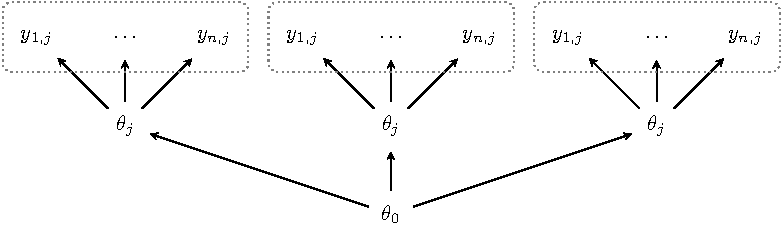
\includegraphics[scale=.65]{../../manuscript/figures/dag-partialpool.pdf}  
    \caption{ Graph depicting the general structure for the hierarchical models, for one populatoin. Observations from each year, $y_{ij}$, are shown grouped and outlined by dotted lines. The observations are drawn from year-level parameters, $\theta_j$, which in turn are drawn from a population-level parameter, $\theta_0$. The graph omits variance terms. }
 \label{fig:hierarchical-dag}
%\end{figure}
\end{wrapfigure}

The distribution of the observations $y_{ij}$ is conditional on the year-specific parameters $\theta_j$ and $\sigma^2_j$. In turn, the year-specific parameter $\theta_j$ is conditional on the population-specific parameters $\theta_0$ and $ \varsigma^2$. We placed priors on all parameters found only on the right hand side of conditional statements ($\theta_0, \sigma^2_j, \varsigma^2$). In practice, we implemented this model by specifying the population- and year-levels of the model with normal distributions; for example, $[ \theta_j | \theta_0 , \varsigma^2 ]$ is $\theta_j \sim N(\theta_0, \varsigma^2)$. The model thus describes a structure in which years are nested within populations.

\subsection{Joint model for seed vital rates}

We estimated the probabilities that seeds germinate, remain intact in the soil seed bank, and survive from seed production to the first October. We constructed models for (1) age-specific germination, (2) persistence of intact seeds, and (3) emergence of seedlings in permanent plots. We then linked these models to jointly estimate seed-related vital rates (Figure \ref{fig:dag-seed-bag}). The posterior and proportional joint distribution for the full model and choices for priors are specified in the \hl{Appendix: Posteriors} and \hl{Appendix: Posteriors}, respectively.

Seeds leave the seed bank through mortality or germination, and remain intact in the seed bank by remaining intact not germinating. In the seed bag burial experiment, we counted intact seeds for up to three years, and counted seedlings after winter rains once per year (Figure \ref{fig:seed-bag-experiments}A). We linked the data by describing survival as the product of a continuous persistence and discrete (absence of) germination survival function (Figure \ref{fig:seed-bag-experiments}A). We thus used the product integral of a continuous and a discrete survival function corresponding to seed survival and not germinating. 

We model age-specific germination with a binomial likelihood and logit-link for the latent probability of germination. The latent probability of germination at each age is described by two hierarchical levels: the first level is the experimental years and the second (upper) level is the population. The discrete component of the survival function is the complement of the age-specific germination probability. 

We model the continuous component of the survival function of intact seeds using a deterministic function. We use a Weibull survival function (\hl{Klein and Moeschberger, Smits 2015}) to model the probability of seed survival after $t$ months. The Weibull survival function is controlled by a shape and scale parameter which determine the shape and rate of the survival trajectory. The Weibull has a shape and scale parameter; we estimate a shape parameter for each population ($\alpha_j$) \hl{Smits 2015}. This is equivalent to assuming the rate of change in survivorship is a population-level property but that the scale varies from year to year within each population ($\eta_{ijk}$). The scale parameter is described by two hierarchical levels: the first level is the experimental year and the second (upper) level is the population.

We then combined the continuous component of the survival function, and used the complement of age-specific germination probabilities to obtain the discrete survival function describing seeds remaining in the seed bank. We model the persistence of intact seeds with a binomial likelihood and logit-link for the latent probability. The latent probability of germination at each observation instance is described by the product of the continuous and discrete components of the survival function. 

We modeled seed survival like this for a few reasons. First, it allowed us to use all of the data from the seed bag experiments at once. Second, it reduced the number of parameters to estimate. Third, it allowed us to reconcile variation in observations and process: seed counts could increase from one observation period to the next and the model could decide what amount of this was due to sampling variation and what was due to the survival process. 

The seed bag burial experiment allowed us to estimate seed fates starting in October after seed production but does not provide direct information about seeds between seed production and the start of the experiment. To estimate the survival of seeds from seed production to October, we augmented the model described so far with one additional component. Briefly, we used estimates for the number of seeds produced in year $t$, seedlings emerging in year $t+1$, and our model for seed survival and germination to infer seed survival from seed production to October. We assumed that the majority of seedlings in a plot emerge from seeds produced the previous year and thus do not model germination from older seeds.

We use the counts of fruits per plant conducted in the permanent plots to get a total number of fruits per plot. We then multiply this count by the average number of seeds per fruit to get an estimate of the number of seeds produced per plot. We do this for aboveground data in 2007 and 2008. We link this data to the number of seedlings observed in the same plots in the following year (2008 and 2009, respectively). We thus take the total number of seeds produced in year $t$ as the number of trials in a binomial experiment for which the outcome is the number of seedlings observed in year $t+1$. The probability is the product of survival from reproduction to October ($s_0$, estimated here), survival from October to January, and germination. We have estimates of the latter two probabilities thanks to the seed bag experiments. We link the three components and estimate the remaining term $s_0$.

We are unable to assess the contribution of seeds from outside the plot to the total number of seeds available. Because the number of seedlings sometimes exceed the total number of seeds, we summed across transects to get counts for the number of seeds and observed seedlings.

\begin{figure}[!h]
       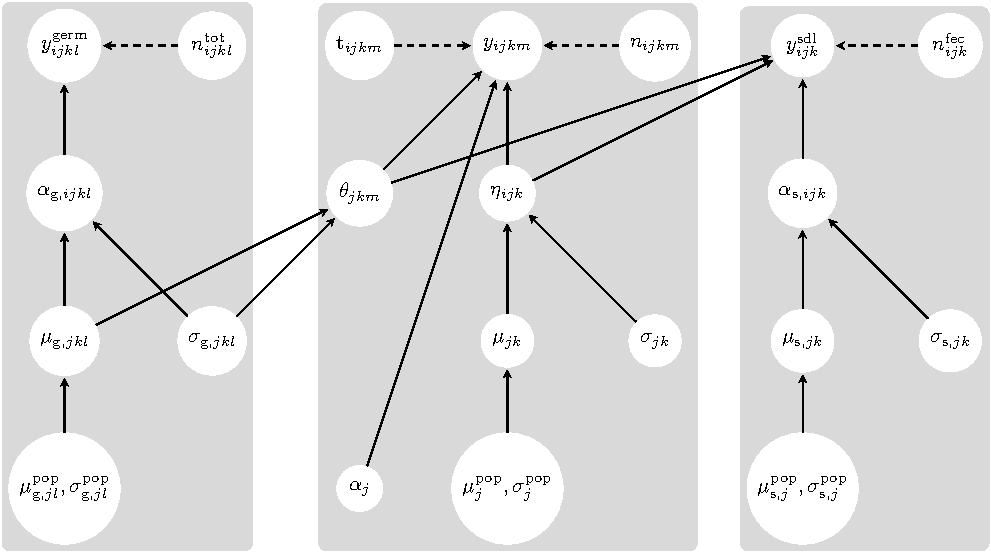
\includegraphics[width=\textwidth]{../../manuscript/figures/dag-seed-bag.pdf}  
    \caption{ Directed acyclic graphs for the full model. Models for each set of data are encapsulated in a gray box; links among the datasets are shown by arrows that cross over between boxes. Solid arrows depict the relationships among random variables, and dashed arrows depict the deterministic relationships. }
 \label{fig:dag-seed-bag}
\end{figure}

\subsection{Viability}

Seeds can also leave the soil seed bank through loss of viability. We estimated viability in a two-stage experiment each October after seed bags were unearthed for a second time (Figure \ref{fig:dag-seed-bag}C). 

All data from viability trials is in the form of binomial trials: we have counts of seeds at the start and end of an experimental window of time. All models have the same structure for seeds in bag $i$ in population $j$ in experimental year $k$. If the number of seeds starting the trial (trials) is $n_{ijk}$ and the number of seeds at the end of the trial (successes) is $y_{ijk}$, we write a model that has a population-level mean and year-level means drawn from the population-level distribution. Broadly, this is two-level hierarchical model with a population-level mean, and year-level means drawn from the population-level distribution. The probability of success for each bag is drawn from this year- and population-level distribution. The model uses a binomial likelihood. 

\subsection{Seedling survival to fruiting}

\begin{wrapfigure}[]{r}{0.25\textwidth}
       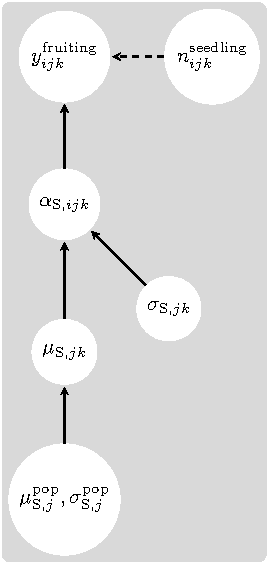
\includegraphics[scale=1]{../../manuscript/figures/dag-survival.pdf}  
    \caption{ Directed acyclic graphs for the model for seedling survival to fruiting. }
 \label{fig:dag-survival}
\end{wrapfigure}

Seedlings can perish from a multitude of causes including end-of-season drought (\hl{Geber and Eckhart 2005}), intra- and interspecific competition (e.g. \hl{Geber and Eckhart 2005, James et al. 2020} small mammal herbivory (\hl{Benning et al. 2019}), and fungal rust morality (\hl{Geber and Eckhart 2005}). To describe variation in survival, we wrote a model that has a population-level mean and year-level means drawn from the population-level distribution. Seedling survival to fruiting (probability of success) for each plot is drawn from this year- and population-level distribution. The model has a binomial likelihood, and thus has a similar structure as the model for data on seed survival.

We obtain the population- and population-by-year posterior distributions of seedling survival to fruiting ($\sigma$) by marginalization. We transform these posteriors to $[0,1]$ by taking the inverse logit; this transforms the parameters into the probability of success.

%\hl{Address missing years, low data years, pooling}

\subsection{Fruits per plant \& seeds per fruit}

Seed production is the product of flowering, (self-)pollination, fruit production, and successful seed set. To describe variation in seed production, we constructed models with population-level mean and year-level means drawn from the population-level distribution. We independently modeled 3 fruit counts (total fruit equivalents, 2006-2012; undamaged fruits, 2013-\hl{present}; damaged fruits, 2013-\hl{present}) and 2 seed counts (seeds per undamaged fruit, 2006-\hl{present}, seeds per damaged fruit, 2013-\hl{present}). We used a Poisson likelihood with a log-link. We modeled sampling uncertainty with a lognormal, which draws the true number of fruits (the $z$s) from a distribution with the median ($\mu$). Each combination of year and population is assigned its own sampling variance ($\sigma^2$). Fruit and seed counts were overdispersed (\hl{show in supplement?}), which the hierarchical structure of the model accommodates with each observation having a unique mean $\lambda$ drawn from a population- and year-specific distribution (\hl{Hobbs and Hooten 2015, p. 253}). 

% Note: Does this make sense? If I'm trying to estimate seed production would it make more sense to model the dataset as is and simply get total seed production in each year as TFE*US (2006-2012), UF*US + DF*DS (2013-2018)?

%Visual inspection of the data on total fruit equivalents (2006--2012) per plant suggests these counts are overdispersed. To assess what probability distribution to use when fitting this model, I fit a power model with an intercept to the mean and variance using the \textbf{nls} function in R, which returned an exponent of 1.85. The fit is close to quadratic which means a negative binomial is likely to be an appropriate distribution (\cite{linden2011}). 

\begin{figure}[!h]
       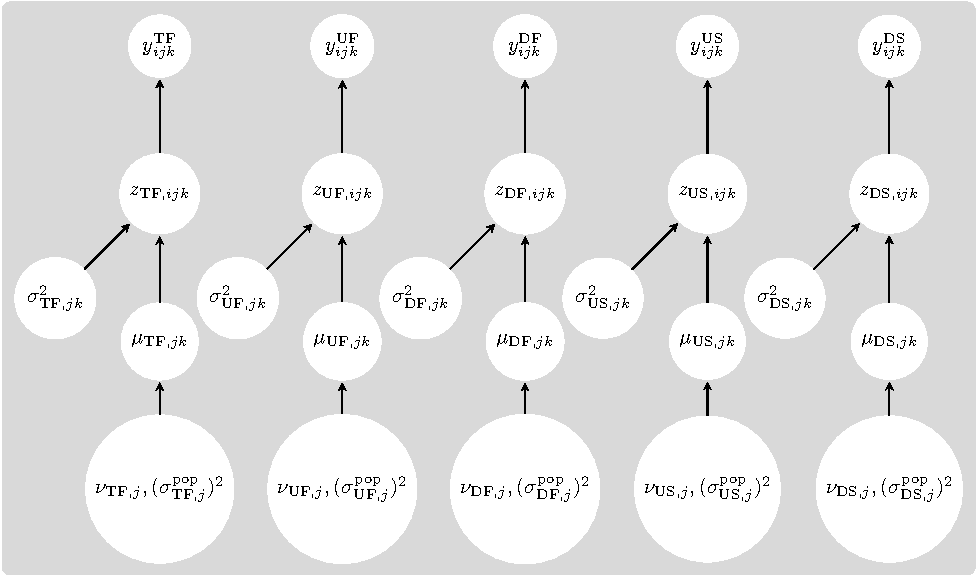
\includegraphics[scale=1]{../../manuscript/figures/dag-fecundity.pdf}  
    \caption{ Directed acyclic graphs for the models for fecundity. }
 \label{fig:dag-fecundity}
\end{figure}

%Visual inspection of the data on undamaged fruits per plant (2013--2018) per plant suggests these counts are overdispersed. To assess what probability distribution to use when fitting this model, I fit a power model with an intercept to the mean and variance using the \textbf{nls} function in R, which returned an exponent of 1.97. The fit is close to quadratic which means a negative binomial i

%\hl{To assess what probability distribution to use when fitting this model,} I fit a power model with an intercept to the mean and variance using the \verb|nls| function in R, which returned an exponent of 1.38. The fit is greater than linear but less than quadratic which means that neither a Poisson nor negative binomial are likely to be entirely appropriate distributions for the data (\cite{linden2011}). I might try the parameterization in that reference but for now I am using the negative binomial because the data are overdispersed. 

\section{Model statements, implementation, and fitting}

We include the expression for the posterior proportional to the joint distribution, and corresponding directed acyclic graphs, in \hl{Appendix: Joint Posterior}. Priors for all parameters are defined in \hl{Table Priors}. We applied the following principles for specifying priors: (1) we used weakly informative priors that avoided placing probability mass on biologically implausible values (\hl{Gelman; Lemoine; Wesner and Pomeranz}), (2) we placed positive, unbounded priors on variance components (\hl{REF}), (3) we conducted prior predictive checks to assess the scale of priors after parameter transformation (\hl{Hobbs and Hooten; Gabry; Wesner and Pomeranz}), and (4) we simulated prior predictive distributions to confirm that the joint likelihood generated data within the observed range (\hl{Gabry; Conn; Hobbs and Hooten}). We provide additional detail regarding our choice of priors in \hl{Appendix: Priors}. 

We prepared data for analysis using the tidyverse and tidybayes packages (\hl{CITE}) in R \hl{VERSION; CITE}. We wrote, fit all models, and estimated posterior distributions using JAGS \hl{VERSION} with rjags (\hl{Plummer 2016}). We randomly generated initial conditions for all parameters with a prior by drawing from the corresponding probability distribution in R before passing the initial values to rjags. We ran three chains for \hl{XX,000} iterations. The first \hl{XX,000} samples were discarded as burn-in and we sampled the following \hl{XX,000} iterations. \hl{We did not thin the chains (Elderd and Miller 2016)}.

We assessed convergence of the MCMC samples with visual inspection of trace plots, by calculating the Brooks-Gelman-Rubin diagnostic (R-hat), and by calculating the Heidelberg-Welch diagnostic (\hl{Elderd and Miller 2016}. The Gelman-Rubin diagnostic is used to assess convergence between chains and the Heidelberg-Welch for stationarity within chains. Trace plots for all chains, histograms of R-hat, and the percentage of chains that passed the HW test are shown in the appendix. 
 
To evaluate our model's fit to the data, we performed model checks that are described in full in \hl{Appendix: Model Checking}. We used our posterior distribution to simulate replicate datasets based on the parameters of our model. We compared samples from the simulated datasets to the real, observed datasets using both graphical, visual checks and by calculating Bayesian \textit{p}-values for test statistics calculated for the observed and simulated data. In the following section, we describe how we used the models we fit to obtain the parameters that describe the \textit{Clarkia} life history. While we do not perform model checks for these derived quantities (e.g. winter seed survival accounting for the combined effect of seed decay and loss of viability) because we combine the output of multiple models, the model checks are still essential to determine whether our inferences are reasonable.

\section{Computing vital rates}

\subsection{Belowground vital rates - seed bank paper}

We used the age-specific germination probabilities, survival function, and viability estimates to account for viability in estimates for the probability of germination and survival. We first discretized the survival function to times at which we observed germination and counted seeds (January and October). Estimates of survival over these intervals are the probability that a seed remains intact, but does not account for loss of viability. Next, we used viability estimates from October to calculate viability for January by interpolation (Figure \ref{fig:seed-bag-experiments}D). We tested the viability of seeds in October, and were thus able to estimate the proportion of viable seeds (Figure \ref{fig:seed-bag-experiments}B; filled points). We inferred the viability of intact seeds in January by assuming that seeds lost viability at a constant rate (exponential decay). Further, we interpolated between estimates by assuming that viability changed at a constant rate between years, and that all seeds were viable at the start of the experiment (Figure \ref{fig:seed-bag-experiments}B; open points). 

We combined the discretized survival function and viability estimates to construct a survival function for the probability that a seed remains intact and viable (Table \ref{tab:survival-functions}, \hl{column X}). Specifically, we multiplied the posteriors of the discretized survival and viability estimates. Because we combined estimates, some portions of the posterior for seed survival probability was than 1, especially for later seed ages. We restricted the posterior to be less than 1 by truncating the distribution and resampling to redistribute the probability mass. We take this step to retain parameter uncertainty about survival probability in cases where combining the estimates implies a high probability of survival. The survival function for viable seeds ($\phi$) is composed of estimates of persistence over time ($\theta_\cdot$), estimates of viability ($\nu_\cdot$), and estimates of germination conditional on persistence ($\gamma_\cdot$).

We used the discretized survival function and age-specific germination probability to obtain the estimates of germination and seed survival required to test predictions from bet-hedging theory. Table \ref{tab:structured-parameters} defines the age-specific germination probabilities and survival probabilities for the structured model in \hl{Eckhart et al. 2011} in terms of the survival function and age-specific germination probabilities. Figure \ref{fig:seed-bag-experiments}E-F illustrate the relationship among the various probabilities of germination and seed survival. Estimates from the seed bag experiment correspond to the probability of germination or survival conditional on persistence (e.g. $\gamma_1$). Multiplying these estimates by the probability of persistence up to a certain time gives the unconditional probability (e.g. $\theta_1 \times \gamma_1$). Finally, the probability conditional on persistence and viability is estimated by incorporating loss of viability into the survival function (e.g. $\gamma_1 / \phi_1$), and defines the parameters in the structured population model.

\singlespace
%
\begin{center}
\captionof{table}{ Seed persistence and viability in the soil seed bank } \label{tab:survival-functions} 
 \begin{tabularx}{11cm}{l  | c | l    } 
  \multicolumn{1}{ c | }{  } & 
  \multicolumn{1}{ c |  }{ Persistence } & 
   \multicolumn{1}{ c  }{ Persistence \& viability } \\ 
 \hline
 \hline
 \multicolumn{1}{ l }{ Time $(x_i)$ } & 
\multicolumn{1}{ | c | }{ $S(x_i)$ } & 
 \multicolumn{1}{ c }{ $S(x_i)$ } \\
 \hline

 $\mathrm{Oct_0}$ & $\theta_0$ & $\phi_0 =  \theta_0$  \\

  $\mathrm{Jan_{1,total}}$ & $\theta_1$ & $\phi_1 = \theta_1 (\gamma_1 + (1-\gamma_1) \nu^{1/3}_1 ) $   \\

  $\mathrm{Jan_{1,intact}}$ & $\theta_2$ & $\phi_2 = \theta_2 \nu^{1/3}_1$  \\

   $\mathrm{Oct}_1$ & $\theta_3$ & $\phi_3 = \theta_3 \nu_1$  \\

  $\mathrm{Jan_{2,total}}$ & $\theta_4$ & $\phi_4 = \theta_4 (\gamma_2 + (1-\gamma_2) \nu_1 (\nu_2 / \nu_1 )^{1/3}) $ \\
  
  \hline
 \hline
 \multicolumn{1}{ l }{ Description  } & 
\multicolumn{1}{ | c | }{ Parameter } & 
 \multicolumn{1}{ c }{ Probability } \\
 \hline
  
July-October & $s_0$ &  \\

October-January & $s_1$ & $ \phi_1$ \\

1-year old germination &  $g_1$  & $  \gamma_1  / \phi_1 $ \\

January-October & $s_2$ &  $ \phi_3 / \phi_2 $  \\

October-January & $s_3$ & $  \phi_4 / \phi_3  $ \\
 
  \hline
   \hline
 
  \hline
\end{tabularx}
\end{center}
%
\doublespace

\subsection{Per-capita reproductive success}

In order to make our analysis comparable to previous empirical studies of bet hedging, we calculated per-capita reproductive success as the product of the probability of seedling survival to fruiting, fruits per plant, and seeds per fruit. We thus calculate per-capita reproductive success as the number of seeds produced per seedling, on average (e.g. \hl{Venable 2007, Gremer et al. 2014}). 

We used a consistent method to estimate seedling survival to fruiting throughout the experiment, and use the population- and year-level means ($\mu_{\mathrm{S},jk}$) in our calculation. Because we estimated fruit production in 2 different ways during the study, we chose to use total fruit equivalents (TFE) per plant as our common estimate of fruit production. From 2006--2012, we used $\mu_{\mathrm{TFE},jk})$ as estimated in the statistical model. From 2013--\hl{2018}, we used the ratio of seeds per damaged to undamaged fruit to calculate a proportion of damaged fruits to add to undamaged fruit counts, as in 

\begin{align}
\begin{split}
\textrm{TFE} = \textrm{undamaged fruits} + \frac{\textrm{seeds per damaged fruit}}{\textrm{seeds per undamaged fruit}}\times  \textrm{damaged fruits} .
  \end{split}
\end{align}

We used posterior distributions for population- and year-level parameters (e.g. $\mu_{\mathrm{US},jk}$) for these calculations and obtained estimates of $\mu_{\mathrm{TFE},jk})$ for 2013--\hl{2018}. Finally, we used estimates of seeds per undamaged fruit ($\mu_{\mathrm{US},jk}$) as our estimate of seeds per fruit.

In terms of parameters from our statistical models, per-capita reproductive success $F_{jk}$ at population $j$ in year $k$ is calculated as

\begin{align}
  \begin{split}
F_{jk} = \phi_{jk} \times \lambda_{\mathrm{TFE},jk} \times \lambda_{\mathrm{US},jk}, \label{eq:percapitars}
  \end{split}
\end{align}

where

\begin{align}
  \begin{split}
\phi_{jk} & = \mathrm{logit}^{-1}(\mu_{\mathrm{S},jk}) \\
\lambda_{\mathrm{TFE},jk} & = \mathrm{exp}(\mu_{\mathrm{TFE},jk}) \\
\lambda_{\mathrm{US},jk} & = \mathrm{exp}(\mu_{\mathrm{US},jk}). 
  \end{split}
\end{align}

Our multilevel models for aboveground vital rates pooled data more strongly in years with relatively little data. A benefit of this approach is that it implicitly corrects for variation in sample size (e.g. an observation of 0/37 seeds surviving is given more weight than an observation of 0/1 seeds surviving). While this is beneficial for distinguishing between spurious estimates and true temporal variation in reproductive success, it may also underestimate variation in reproductive success. At the extreme, estimates in years without any data are pooled to the population-level means. Years with zero seedling survivorship would thus have estimates for fruits per plant that are pooled towards the population-mean (because there were no fruiting plants on which to count fruits). 

\iffalse

We calculated the posterior mode of annual estimates for each parameter in \hl{Equation 6} before multiplying to obtain the per-capita reproductive success in that year. Using the posterior mode is equivalent to taking the BLUP of a linear model, and allowed us to estimate vital rates in years with small sample sizes. 

\hl{WORK ON THIS}


We decided to deal with this issue by considering a second, less strict test. We took the years in which we observed zero plants or no survivorship in permanent plots (even if there were plants elsewhere in the population) and did the following. First, if we observed zero plants we calculated the probability of no germination given the number of seeds that were produced the previous year. To do this, we used the estimates of fruits per plant and seeds per fruit to estimate the average number of seeds produced per plot in each population. We then multiplied this by s0, s1, and g1. We used the population-level estimates for these calculations. Specifically, we asked what the probability of observing no germination was given the population-level estimates of s0*s1*g1.

Second, if we observed no survivorship we calculated the probability of no survivorship given the number of seedlings. We took the plots and repeated binomial trials at each plot until we arrived at the probability of survival necessary to get the observed 0 survivorship. 

Rather than assume that survival probability was 0 we sought to get a 90\% probability of no survivorship or germination. 




%Describe dealing with missing years (compare to Venable)

%Describe selecting combinations of parameter estimates from each year (for all 3 rates).

%Describe using the posteriors to calculate ratio of and get TFE equivalents in later years. 



\clearpage
\newpage

\begin{singlespace*}...
\captionof{table}{ Summary of zeros and missing data in Venable 2007. } \label{tab:venable} 
\begin{center}
 \begin{tabular}{ l c c c c  c } 
 \hline
 \hline
\multicolumn{1}{ l }{ Description  } &
\multicolumn{1}{ c }{ Seedlings } & 
\multicolumn{1}{ c }{ Fruiting plants } & 
\multicolumn{1}{ c }{ lx }  & 
\multicolumn{1}{ c }{ bx  }  & 
\multicolumn{1}{ c }{ lx bx }  \\
 \hline
 % seed bag burial experiment
No survival; 0 fitness  & \# & 0 & 0 & NA & 0  \\
No germination; 0 fitness & 0 & 0 & NA & NA & 0  \\
Missing data & \# & \# & \# & NA & NA   \\
   \hline
\end{tabular} 
\end{center}
\end{singlespace*}

Units for lx are (plants/seedling), for bx are (seeds/plant), and for lxbx are (seeds/seedling). To analyze the variance in per capita reproductive success, Venable (2007) added 0.5 to per capita reproductive success before taking the log. 


Our dataset is a bit different because we have and use data both from permanent plots and additional surveys. So, if seedling survival to fruiting is 0 in plots or there is no germination, we still might observe plants elsewhere in the population. 


\begin{singlespace*}...
\captionof{table}{ Summary of zeros and missing data in Venable 2007. } \label{tab:venable} 
\begin{center}
 \begin{tabular}{ l c c c c  c } 
 \hline
 \hline
\multicolumn{1}{ l }{ Description  } &
\multicolumn{1}{ c }{ Seedlings } & 
\multicolumn{1}{ c }{ Fruiting plants } & 
\multicolumn{1}{ c }{ Fruits per plant }  & 
\multicolumn{1}{ c }{ Seeds per fruit  }  & 
\multicolumn{1}{ c }{ lx bx }  \\
 \hline
 % seed bag burial experiment
0 survival in plots & \# & 0 & \# & \# & \dots  \\
0 survival in plots, throws & \# & 0 & NA & NA & 0  \\
0 seedlings in plots & 0 & 0 &  \# & \# & \dots \\
0 seedlings in plots, throws & 0 & 0 &  NA & NA & 0 \\
missing data & \# & \# & \# & NA & NA   \\
   \hline
\end{tabular} 
\end{center}
\end{singlespace*}

Units for survival are (fruiting plants/ seedling), for bx are the product of fruits per plant and seeds per fruit to get (seeds/fruiting plant) and then per-capita RS is lxbx which has units (seeds/seedling).

We test the predictions of the density-independent model using two levels of stringency. The strong test of the model uses the hierarchical model, with partially pooling, to estimate reproductive success. We consider this the strict test because estimates of reproductive success are corrected for sampling variation (partial pooling) and years without data are pooled towards the population-means. This is certainly beneficial for distinguishing between spurious estimates and true temporal variation in reproductive success; however, it may also underestimate variation in reproductive success if there is correlation between components of the life cycle. Because we model each component of reproductive success separately, our estimates are pooled to the population-mean for the vital rate. Years with zero seedling survivorship would thus have estimates for fruits per plant that are pooled towards the population-mean (because there were no fruiting plants on which to count fruits). This would be okay if we estimated low survivorship; but if we had few seedlings in which to observe survivorship then those estimates would also be pooled. 


We decided to deal with this issue by considering a second, less strict test. We took the years in which we observed zero plants or no survivorship in permanent plots (even if there were plants elsewhere in the population) and did the following. First, if we observed zero plants we calculated the probability of no germination given the number of seeds that were produced the previous year. To do this, we used the estimates of fruits per plant and seeds per fruit to estimate the average number of seeds produced per plot in each population. We then multiplied this by s0, s1, and g1. We used the population-level estimates for these calculations. Specifically, we asked what the probability of observing no germination was given the population-level estimates of s0*s1*g1.

Second, if we observed no survivorship we calculated the probability of no survivorship given the number of seedlings. We took the plots and repeated binomial trials at each plot until we arrived at the probability of survival necessary to get the observed 0 survivorship. 

Rather than assume that survival probability was 0 we sought to get a 90\% probability of no survivorship or germination. 

\clearpage
\newpage

\fi


\clearpage
%%%%%%%%%%%%%%%%%%%%%%%%%%%%%%%%%%%%%%%%%%%%%%%%%%%%
% BIBLIOGRAPHY
%%%%%%%%%%%%%%%%%%%%%%%%%%%%%%%%%%%%%%%%%%%%%%%%%%%%
\bibliographystyle{/Users/gregor/Dropbox/bibliography/styleFiles/ecology} 
\bibliography{/Users/gregor/Dropbox/bibliography/chapter-1}

\end{document}